% Drawing a graph
% Author: Stefan Kottwitz
% https://www.packtpub.com/hardware-and-creative/latex-cookbook
\documentclass[border=10pt]{standalone}
\usepackage{tkz-graph}
\usepackage{tikz}
\usetikzlibrary{positioning}

%\GraphInit[vstyle = Shade]
%\tikzset{
%  LabelStyle/.style = { rectangle, rounded corners, draw,
%                        minimum width = 2em,
%                        text = black, font = \bfseries },
%  VertexStyle/.append style = { inner sep=5pt,
%                                font = \Large\bfseries},
%  EdgeStyle/.append style = {->, bend left} }
%\thispagestyle{empty}
\begin{document}
%\begin{tikzpicture}
%  \SetGraphUnit{5}
%  \Vertex{B}
%  \WE(B){A}
%  \EA(B){C}
%  \Edge[label = 1](A)(B)
%  \Edge[label = 2](B)(C)
%  \Edge[label = 3](C)(B)
%  \Edge[label = 4](B)(A)
%  \Loop[dist = 4cm, dir = NO, label = 5](A.west)
%  \Loop[dist = 4cm, dir = SO, label = 6](C.east)
%  \tikzset{EdgeStyle/.append style = {bend left = 50}}
%  \Edge[label = 7](A)(C)
%  \Edge[label = 8](C)(A)
%\end{tikzpicture}




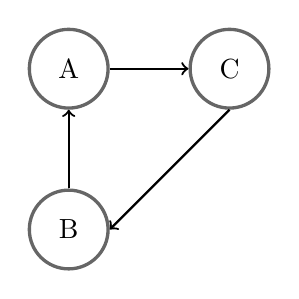
\begin{tikzpicture}[
roundnode/.style={circle, draw=black!60,  very thick, minimum size=10mm},
squarednode/.style={rectangle, draw=red!60, fill=red!5, very thick, minimum size=5mm},
]
%Nodes
\node[roundnode]      (A)                    {A};
\node[roundnode]      (B)       [below=of A] {B};
\node[roundnode]      (C)       [right=of A] {C};

 
%Lines
\draw[thick,->] (B.north) -- (A.south);
\draw[thick,->] (A.east) -- (C.west);
\draw[thick,->]  (C.south) -- (B.east);
%\draw[->] (C.south) .. controls +(down:7mm) and +(right:7mm) .. (A.east);
\end{tikzpicture}


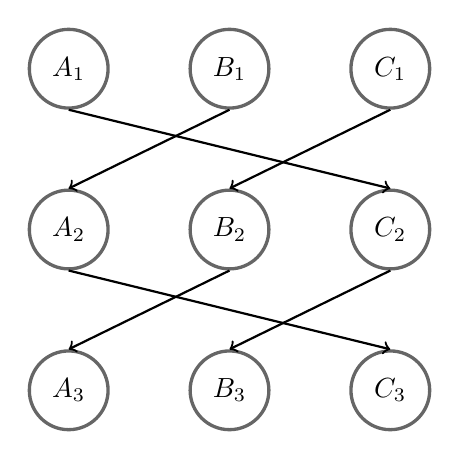
\begin{tikzpicture}[
roundnode/.style={circle, draw=black!60,  very thick, minimum size=10mm},
squarednode/.style={rectangle, draw=red!60, fill=red!5, very thick, minimum size=5mm},
]
%Nodes
\node[roundnode]      (A1)                    {$A_1$};
\node[roundnode]      (B1)       [right=of A1] {$B_1$};
\node[roundnode]      (C1)       [right=of B1] {$C_1$};

\node[roundnode]      (A2)       [below=of A1]             {$A_2$};
\node[roundnode]      (B2)       [right=of A2] {$B_2$};
\node[roundnode]      (C2)       [right=of B2] {$C_2$};

\node[roundnode]      (A3)       [below=of A2]             {$A_3$};
\node[roundnode]      (B3)       [right=of A3] {$B_3$};
\node[roundnode]      (C3)       [right=of B3] {$C_3$};
 
%Lines
\draw[thick,->] (A1.south) -- (C2.north);
\draw[thick,->] (B1.south) -- (A2.north);
\draw[thick,->] (C1.south) -- (B2.north);

\draw[thick,->] (A2.south) -- (C3.north);
\draw[thick,->] (B2.south) -- (A3.north);
\draw[thick,->] (C2.south) -- (B3.north);


\end{tikzpicture}


\end{document}

